\section{Differential Equations}
\label{sec:diff-eqs}
% From Section 3.8
% This section needs a lot of graphics.

A {\bf differential equation}\index{Differential equation} is an equation involving the derivative of a function. They allow us to express with a simple equation the relationship between a quantity and it's rate of change.

\begin{example}
A bank pays 2\% interest on its certificate of deposit accounts, but charges a \$20 annual fee. Write an equation for the rate of change of the balance, $B'(t)$.

\begin{solution}
  If the balance $B(t)$ has units of dollars, then $B'(t)$ has units of dollars per year. When we think of what is changing the balance of the account, there are two factors:
\begin{enumerate}
  \item The interest, which increases the balance, and
  \item The fee, which decreases the balance.
\end{enumerate}
Considering the interest, we know each year the balance will increase by 2\%, but 2\% of what? Each year that will change, since we earn interest on whatever the current balance is. We can represent the amount of increase as 2\% of the balance: $0.02B(t)$ dollars/year.

The fee already has the units of dollars/year. Since everything now has the same units, we can put the two together, and create the equation:
$$B'(t)=0.02B(t)-20 \enspace .$$
\end{solution}\end{example}

The result is an example of a differential equation. Notice this particular equation involves both the derivative and the original function, and so we can't simply find $B(t)$ using basic integration.

Algebraic equations contain constants and variables, and the solutions of an algebraic equation are typically numbers. For example, $x=3$ and $x=-2$ are solutions of the algebraic equation $x^2=x+6$. Differential equations contain derivatives or differentials of functions. Solutions of differential equations are functions. The differential equation $y'=3x^2$ has infinitely many solutions, and two of those solutions are the functions $y=x^3+2$ and $y=x^3-4$.

\begin{figure}[!ht]
  \centering
    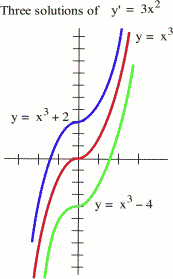
\includegraphics[width=0.4\textwidth]{img/chap5/image064.png}
    \caption{Three solutions to $y'=3x^2$.}
    \label{fig:5-9-solutioncurves}
\end{figure}
You have already solved lots of differential equations: every time you found an antiderivative of a function $f(x)$, you solved the differential equation $y'=f(x)$ to get a solution $y$. The differential equation $y'=f(x)$, however, is just the beginning. Other applications generate different differential equations, like in the bank balance example above.

\subsection{Checking Solutions of Differential Equations}
Whether a differential equation is easy or difficult to solve, it is important to be able to check that a possible solution really satisfies the differential equation.

A possible solution of an algebraic equation can be checked by putting the solution into the equation to see if the result is true: $x=3$ is a solution of $5x+1=16$ since $5(3)+1=16$ is true. Similarly, a solution of a differential equation can be checked by substituting the function and the appropriate derivatives into the equation to see if the result is true: $y=x^2$ is a solution of $xy'=2y$ since $y'=2x$ and $x(2x)=2(x^2)$ is true.

\begin{example}
Verify the following.
  \begin{enumerate}[label=(\alph*)]
    \item $y=x^2+5$ is a solution of $y''+y=x^2+7$.

    \begin{solution}
      $y=x^2+5$ so $y'=2x$ and $y''=2$. Substituting these functions for $y$ and $y''$ into the differential equation $y''+y=x^2+7$, we have
        $$y''+y=(2)+(x^2+5)=x^2+7 \enspace ,$$
    so $y=x^2+5$ is a solution of the differential equation.
    \end{solution}

    \item $y=x + \dfrac{5}{x}$ is a solution of $y' + \dfrac{y}{x}=2$.

    \begin{solution}
    $y=x+\dfrac{5}{x}$ so $y'=1-\dfrac{5}{x^2}$. Substituting these functions for $y$ and $y'$ in the differential equation $y'+\dfrac{y}{x}=2$, we have
    $$y' + \dfrac{y}{x} = \left(1-\dfrac{5}{x^2}\right) + \dfrac{1}{x}\left(x + \dfrac{5}{x}\right) = 1 - \dfrac{5}{x^2} + 1 + \dfrac{5}{x^2} = 2 \enspace ,$$
    the result we wanted to verify.

    \end{solution}
  \end{enumerate}
\end{example}

\subsection{Separable Differential Equations}
A differential equation is called {\bf separable}\index{Differential equation!separable} if the variables can be separated algebraically so that all the $x$'s and $dx$ are one one side of the equation, and all the $y$'s and $dy$ are on the other side of the equation. In other words, the differential equation can be written in the form $f(x)\,dx = g(y)\,dy$.

Once separated, separable differential equations can be solved by integrating both sides of the equation.

\begin{example}
Find the solution of
$$y'=\frac{6x+1}{2y} \enspace .$$

\begin{solution}
  Rewriting $y'$ is a helpful first step:
$$\frac{dy}{dx} = \frac{6x+1}{2y} \enspace .$$
Now we can multiply both sides by $dx$ and by $2y$ to separate the variables:
$$ 2y\, dy = (6x+1)\, dx \enspace .$$

Integrating each side, we have
\begin{align*}
  \int 2y\,dy &= \int (6x+1)\,dx \\
  y^2+C_1     &= 3x^2+x+C_2
\end{align*}
Notice that we can combine the two constants to create a new, consolidated constant $C$, so we usually only bother to put a constant on the right side:
$$y^2 = 3x^2+x + C \enspace .$$
\end{solution}\end{example}

As expected, there is a whole family of solutions to this differential equation.

\begin{definition}[Initial Value Problem (IVT)]
An {\bf initial value problem}\index{Initial value problem} is a differential equation that provides additional information about specific values of the function and/or one or more of its derivatives. Often, the specific values will be initial values, that is, when $x=0$. This allows us to then solve for the constant and find a single solution.
\end{definition}

\begin{example}
Find the solution of $y'=\dfrac{6x+1}{2y}$ which satisfies $y(2)=3$.

\begin{solution}
  In the previous example we found the general solution, $y^2=3x^2+x+C$.

Substituting in the initial condition, $y=3$ when $x=2$,
$$3^2=3(2)^2+2+C \enspace ,$$
so $9=12+2+C$, giving $C=-5$.

The solution is
$$y^2=3x^2+x-5 \enspace .$$
Sometimes it is desirable to solve for $y$, which would yield $y=\pm\sqrt{3x^2+x-5}$, but since the initial condition had a positive $y$ value, we isolate the positive solution:
$$y=\sqrt{3x^2+x-5} \enspace .$$
\end{solution}\end{example}

\begin{example}
A bank pays 2\% interest on its certificate of deposit accounts, but charges a \$20 annual fee. If you initially invest \$3,000, how much will you have after 10 years?

\begin{solution}
  You may recognize this as the example from the beginning of the section, for which we set up the equation $$B'(t)=0.02B(t)-20$$ or, more simply,
$$\frac{dB}{dt}=0.02B-20 \enspace .$$
We can separate this equation by multiplying by $dt$ and dividing by the entire expression on the right:
$$\frac{dB}{0.02B-20}=dt \enspace .$$
Integrating the left side of this equation requires substitution. Let $u=0.02B-20$, so $du=0.02\,dB$. Making the substitution,
\begin{align*}
  \int \frac{dB}{0.02B-20} &=\int \frac{du/0.02}{u} \\
    &= \int \frac{1}{u}\frac{du}{0.02} \\
    &= \frac{1}{0.02}\int \frac{1}{u}\,du \\
    &= \frac{1}{0.02}\ln|u| + C_1 \\
    &= \frac{1}{0.02}\ln|0.02B-20| + C_1
\end{align*}
Integrating on the right side of the differential equation is easier:
$$\int dt=t+C_2 \enspace .$$
Together, this gives us the general solution to the differential equation (we're also combining the $C$'s in this step):
$$\frac{1}{0.02}\ln|0.02B-20|=t+C \enspace .$$
Now we would like to solve for $B$. Start by multiplying by 0.02.

\begin{align*}
\ln|0.02B-20|     &= 0.02t+0.02C  \\
\ln|0.02B-20|     &= 0.02t+D      & \text{Let }D=0.02C\\
e^{\ln|0.02B-20|} &= e^{0.02t+D}  & \text{Exponentiate both sides}\\
|0.02B-20|        &= e^{0.02t+D}  & \text{Use the log rule: } e^{\ln(A)}=A.\\
0.02B-20          &= e^{0.02t+D}  & \text{The right side is positive.}\\
0.02B-20          &= e^{0.02t}e^D & \text{Use the rule: } e^{A+B}=e^Ae^B.\\
0.02B-20          &= ke^{0.02t}   & \text{Let } k=e^D\\
0.02B             &= ke^{0.02t} + 20   \\
B                 &= \frac{ke^{0.02t} + 20}{0.02} \\
B                 &= \frac{ke^{0.02t}}{0.02} + 1000 \\
B                 &= Ae^{0.02t}+1000 &= \text{Let } A = \frac{k}{0.02}
\end{align*}
Finally, we can substitute our initial value of $B=3000$ when $t=0$ to solve for the constant $A$:
\begin{align*}
3000  &= Ae^{0.02(0)}+1000 \\
A     &= 2000
\end{align*}
This gives us the equation for the account balance after $t$ years:
$$B(t)=2000e^{0.02t}+1000 \enspace .$$
To find the balance after 10 years, we can evaluate this equation at $t=10$:
$$B(10)=2000e^{0.02(10)}+1000 \approx   \$3442.81 \enspace .$$
\end{solution}\end{example}

It's worth noting that this answer isn't exactly right. Differential equations assume continuous changes, and it is unlikely interest is compounded continuously or the fee is extracted continuously. However, the answer is probably close to the actual answer, and differential equations provide a relatively simple model of a complicated situation.

\subsection{Models of Growth}
The bank account example demonstrated one basic model of growth: growth proportional to the existing quantity. Bank accounts and populations both tend to grow this way if not constrained. This type of growth is called unlimited growth.

\begin{definition}[Unlimited Growth]
If a quantity or population $y$ grows at a rate proportional that quantity's size, it can be modeled with {\bf unlimited growth}\index{Unlimited growth} (also called {\bf unbounded growth})\index{Growth!unbounded}, which has the differential equation:
$$y'=ry \enspace ,$$
where $r$ is a constant.
\end{definition}

\begin{example}
A population grows by 8\% each year. If the current population is 5,000, find an equation for the population after $t$ years.

\begin{solution}
\begin{align*}
  \frac{dy}{dt} &= 0.08y  \\
  \frac{1}{y}\,dy &= 0.08\,dt \\
  \ln|y| &= 0.08t+C \\
  e^{\ln|y|} &= e^{0.08t+C}\\
  y &= Ae^{0.08t}
\end{align*}
  Separate the variables.Integrate both sides.Exponentiate both sides.Simplify both sides, using the tricks we used in the bank example.
Now substitute in the initial condition: $5000=Ae^{0.08(0)}$, so $A=5000$.

The population will grow following the equation
$$y=5000e^{0.08t} \enspace .$$
\end{solution}\end{example}

Notice that the solution to the unlimited growth equation is an exponential equation\index{Function!exponential}.

When a product is advertised heavily, sales will tend to grow very quickly, but eventually the market will reach saturation, and sales will slow. In this type of growth, called {\bf limited growth}, {\bf bounded growth}, or {\bf constrained growth}\index{Limited growth}\index{Bounded growth}, the population grows at a rate proportional to the distance from the maximum value.

\begin{definition}[Bounded Growth]
If a quantity grows at a rate proportional to the distance from the maximum value, $M$, it can be modeled with {\bf bounded growth}, which has the differential equation
$$y'=k(M-y) \enspace ,$$
where $k$ is a constant, and $M$ is the maximum size of $y$.
\end{definition}

\begin{example}
A new cell phone is introduced. The company estimates they will sell 200 thousand phones. After 1 month they have sold 20 thousand. How many will they have sold after 9 months?

\begin{solution}
In this case there is a maximum amount of phones they expect to sell, so $M=200$ thousand. Modeling the sales, $y$, in thousands of phones, we can write the differential equation
$$y'=k(200-y) \enspace .$$
Since it was a new phone, $y(0)=0$. We also know the sales after one month, $y(1)=20$.

Solving the differential equation:
\begin{align*}
  \frac{dy}{dt}         &= k(200-y) \\
  \frac{dy}{200-y}      &= k\,dt        & \text{Separate the variables.}\\
  \int\frac{dy}{200-y}  &= \int k\,dt   & \text{Integrate both sides.}\\
  -\ln|200-y|           &= kt+C         & \text{On the left, use the substitution } u=200-y.\\
  e^{\ln|200-y|}        &= e^{-kt+C}    & \text{Multiply both sides by } -1 \text{ and exponentiate both sides.} \\
  200-y                 &= Be^{-kt}     & \text{Simplify.}\\
  -y                    &= Be^{-kt} - 200 & \text{Subtract 200.}\\
  y                     &= Ae-kt+200    & \text{Divide by }-1, \text{ and simplify.}
\end{align*}
Using the initial condition $y(0)=0$,
$$0=Ae^{-k(0)} + 200 \enspace ,$$
so $0=A+200$, giving $A=-200$.

Using the value $y(1)=20$:
\begin{align*}
  20              &= -200e^{-k\cdot 1}+200 \\
  -180            &= -200e^{-k}             &\text{Subtract 200.}\\
  \frac{180}{200} &= e^{-k}                 &\text{Divide by } -200. \\
  \ln(0.9)        &= \ln\left(e^{-k}\right) = -k & \text{Take the logarithm of both sides.}\\
  k               &= -\ln(0.9) \approx   0.105  & \text{Divide by } -1.
\end{align*}
As a quick sanity check, this value is positive as we would expect, indicating that the sales are growing over time. We now have the equation for the sales of phones over time:
$$A=-200e^{-0.105t}+200 \enspace .$$
Finally, we can evaluate this at $t=9$ to find the sales after 9 months:
$$A(9) = -200e^{-0.105\cdot 9} + 200  \approx   122.26 \text{ thousand phones.}$$
\end{solution}\end{example}

Limited growth is also commonly used for learning models, since when learning a new skill, people typically learn quickly at first, then their rate of improvement slows down as they approach mastery.

Earlier we used unlimited growth to model a population, but often a population will be constrained by food, space, and other resources. When a population grows both proportional to its size, and relative to the distance from some maximum, that is called {\bf logistic growth}\index{Logistic growth}\index{Growth!logistic}. This leads to the differential equation $y'=ky(M-y)$, which is accurate but not always convenient to use. We will use a slight modification. Since solving this differential equation requires integration techniques we haven't learned, the solution form is given.

\begin{definition}[Logistic Growth]
If a quantity grows at a rate proportional to its size and to the distance from the maximum value, $M$, it can be modeled with {\bf logistic growth}\index{Logistic growth}\index{Function!logistic}, which has the differential equation:
$$y' = ry\left(1-\frac{y}{M}\right) \enspace .$$
$r$ can be interpreted as the growth rate absent constraints, i.e., how the population would grow if there wasn't a maximum value.

This differential equation has solutions of the form
$$y = \frac{M}{1+Ae^{-rt}} \enspace .$$
\end{definition}
\begin{example}
A colony of 100 rabbits is introduced to a reclaimed forest. After 1 year, the population has grown to 300. It is estimated the forest can sustain 5000 rabbits. The forest service plans to reintroduce wolves to the forest when the rabbit population reaches 3000 rabbits. When will that occur?

\begin{solution}
The maximum sustainable population was given as $M=5000$. Using the solution form
$$y=\frac{M}{1+Ae^{-rt}}$$
and the initial condition $y(0)=100$ we can solve for $A$:
\begin{align*}
  100       &= \frac{5000}{1+Ae^{-r\cdot 0}} \\
  100       &= \frac{5000}{1+A} \quad \text{Simplify.}\\
  100(1+A)  &= 5000 \quad \text{Multiply both sides by } 1+A.\\
  1+A       &= 50 \quad \text{Divide by 100.}\\
  A         &= 49
\end{align*}
Now, using $y(1)=300$, we can solve for $r$:
\begin{align*}
 300 &= \frac{5000}{1+49e^{-r(1)}} \\
 300(1+49e^{-r}) &= 5000\\
 1+49e^{-r} &= \frac{5000}{300} = \frac{50}{3}\\
 e^{-r} &= \frac{\frac{50}{3}-1}{49} \approx 0.3197 \\
 -r &\approx \ln(0.3197)\\
 r &\approx -\ln(0.3197)\approx   1.1404 \enspace .
\end{align*}
We now have the equation for the population after $t$ years:
$$y = \frac{5000}{1+49 e^{-1.1404t}} \enspace .$$
To answer the original equation, of when the rabbit population will reach 3000, we need to solve for $t$ when $y=3000$:
\begin{align*}
  3000                              &= \frac{5000}{1+49e^{-1.1404t}} \\
  3000\left(1+49e^{-1.1404t}\right) &= 5000\\
  1+49e^{-1.1404t}                  &= \frac{5}{3}\\
  49e^{-1.1404t}                    &= \frac{5}{3} - 1\\
  e^{-1.1404t}                      &= \frac{\frac{5}{3}-1}{49} \approx  0.01361 \\
  t                                 &= \frac{\ln(0.01361)}{-1.1404}\approx   3.77 \text{ years}.
\end{align*}
\end{solution}\end{example}

Logistic growth is also a good model for unadvertised sales. A new product that is not advertised will have sales increase slowly at first, then grow as word of mouth spreads and people become familiar with the product. Sales will level off as they approach market saturation.
